% Festlegen des Dokumententyps
\documentclass[a4paper,twoside]{article}

% Papierformat
\usepackage{a4}

% Deutsche Sprache (Silbentrennung, usw.)
\usepackage[ngerman]{babel}

% Schrifteneinstellungen
\usepackage{lmodern}
\usepackage[T1]{fontenc}
\usepackage{textcomp}

% bessere Matheunterstützung
\usepackage{amsfonts}
\usepackage{amstext}
\usepackage{amsmath}
\usepackage{empheq}

% Kodierung
\usepackage{ucs}
\usepackage[utf8x]{inputenc}

% Grafiken einbinden
\usepackage{graphicx}
\usepackage{color}

% Floats inside Floats
\usepackage{subfig}

% Prevent Floating outside of Section
\usepackage[section]{placeins}

% Nice Header
\usepackage{fancyhdr}

% Clickable URLs and references
\usepackage{hyperref}

% Bibliography
\usepackage[comma,sort&compress]{natbib}

% Proper units
\usepackage{units}

% Custom packages
% Nicer paragraphs
\parskip 12pt
\parindent 0pt
\renewcommand{\arraystretch}{1.2}
\newcommand{\degree}{\ensuremath{^{\circ}}}
\newcommand{\D}[1]{\ensuremath{\mathrm{d}#1}}
\newcommand{\Dfrac}[2]{\ensuremath{\frac{\mathrm{d}#1}{\mathrm{d}#2}}}
\newcommand{\mensch}[1]{\textsc{#1}}
\newcommand{\T}{\textstyle}
\newcommand{\sym}[1]{$ #1 $}
\newcommand{\ret}{$[\hookleftarrow]$}
\newcommand{\q}[1]{\glqq{#1}\grqq}
\renewcommand{\vec}[1]{\boldsymbol{#1}}

%
\begin{document}

\begin{titlepage}

\includegraphics[height=2cm]{georg} \hfill

\normalsize

\vspace{5cm}

\begin{center}
\Large Physikalisches A-Praktikum \\
\Huge Versuch 12 \\[5mm]
{\bf Die spezifische Elektronenladung $\nicefrac{e}{m_e}$}
\end{center}

\normalsize

\begin{table}[!h]
\begin{center}
\subfloat{
  \begin{tabular}{ll}
  Praktikanten: &Julius Strake\\
  &Niklas Bölter\\
  Gruppe: &B006\\
  \end{tabular}
}
\subfloat{
  \begin{tabular}{ll}
  Betreuer: &Johannes Schmidt\\
  Durchgeführt: &14.09.2012\\
  Unterschrift: &\hspace{3cm} \\
  \cline{2-2}
  \end{tabular}
}
\vspace{2.0cm}
\begin{tabular}{lr}
  E-Mail: & \ttfamily niklas.boelter@stud.uni-goettingen.de\\
          & \ttfamily julius.strake@stud.uni-goettingen.de\\
\end{tabular}
\end{center}
\end{table}
\end{titlepage}
\pagestyle{empty}
\clearpage\markboth{}{}\cleardoublepage
\pagestyle{empty}
\tableofcontents
\newpage
\pagestyle{headings}
\section{Einleitung}
In diesem Versuch soll die spezifische Elektronenladung bestimmt werden.
Hierzu wird ein Elektronenstrahl in einem möglichst homogenen Magnetfeld auf eine Kreisbahn gelenkt und aus deren Radius der Wert berechnet.

\section{Theorie}
\subsection{Spezifische Elektronenladung}
In diesem Versuch wird mit Hilfe von \mensch{Helmholtz}-Spulen ein homogenes Magnetfeld erzeugt. Für den magnetischen Fluss $\vec B$ in der Mitte zwischen den Spulen gilt dann: \citep[S.\,91]{Demtroeder-Exp2}
\begin{align}
  B = \frac{8 \mu_0 N I}{\sqrt{125} R}
  \label{eq:B-Feld}
\end{align}
Dabei ist $R$ der Abstand der beiden Spulen sowie ihr Radius (\mensch{Helmholtz}-Bedingung), N ihre Windungszahl und $I$ der durch die Spulen fließende Strom.

Die Elektronen werden durch die Anodenspannung $U$ beschleunigt, haben danach also die kinetische Energie $E = eU$.
\begin{align*}
  & \frac{1}{2} m_e v^2 = e U \\ 
 \Rightarrow \quad & v = \sqrt{\frac{e}{m_e} 2 U}
\end{align*}
Zusätzlich werden sie mit dem auf negativem Potential befindlichen \mensch{Wehnelt}-Zylinder fokussiert.

Danach werden sie im Magnetfeld der \mensch{Helmholtz}-Spulen auf eine Kreisbahn gelenkt. Diese wirkt also als Zentripetalkraft $F_z = \frac{m v^2}{r}$. Gleichsetzen ergibt:
\begin{align}
  \frac{m_e v^2}{r} &= e v B \nonumber\\
  v^2 &= \left(r \frac{e}{m_e} B\right)^2 \nonumber\\
  \frac{e}{m_e} 2 U &= r^2 \frac{e^2}{m_e^2}B^2 \nonumber\\
  \frac{e}{m_e} &= \frac{2U}{r^2 B^2}. 
  \label{eq:SpezLad}
\end{align}
Dabei ist $r$ der Radius der von den Elektronen beschriebenen Kreisbahn.

\section{Durchführung}
Nach dem Aufbau der Versuchsschaltung wird der Raum abgedunkelt und mit Hilfe des in Abbildung~\ref{fig:Aufbau} dargestellten Okulars die Lage des Austrittspunktes der Elektronen aus der Elektronenkanone bestimmt. 
\begin{figure}[htb]
\begin{center}
\def\svgwidth{8cm}
\input{Aufbau.pdf_tex}
\end{center}
\caption{Versuchsaufbau ohne Spannungsquelle. \citep{LP-Spulen}}
\label{fig:Aufbau}
\end{figure}
Anschließend sollte man durch grobes Verändern der Anodenspannung und des Stroms durch die Helmholtz-Spulen überprüfen, in welchen Bereichen eine sinnvolle Messung des Elektronenstrahlradius möglich ist.
Jetzt werden für zwei feste Anodenspannungen je etwa acht Werte bei variiertem Spulenstrom aufgenommen, ebenso für zwei feste Spulenströme bei variierter Anodenspannung.

\section{Auswertung}
Die Bestimmung des Wertes für die spezifische Elektronenladung aus den einzelnen Wertetripeln per Formel~\ref{eq:SpezLad} ergibt die in Tabelle~\ref{tab:Feldstaerke} angegebenen Ergebnisse.

Aus diesen lässt sich nun ein gewichteter Mittelwert berechnen:
\begin{empheq}[box=\fbox]{align*}
  \frac{e}{m_e} &= (1.631 \pm 0.018) \cdot 10^{11} \unitfrac{C}{kg}
\end{empheq}
Die Abweichung vom Literaturwert beträgt etwa $7.3\,\%$.

Zur Fehlerberechnung wurde die Abweichung des zur Strommessung verwendeten Multimeters\footnote{M2012, Fehler im Messbereich: $\pm\unit[21]{mA}$~\citep[S.\,34f]{Anleitung}}, die des zur Spannungsmessung verwendeten Multimeters\footnote{Metramax 12, Fehler im Messbereich: $\pm \unit[2.6]{V}$~\citep[S.\,14]{Metramax}} und eine Abschätzung des Fehlers im Durchmesser genutzt.
Da der Elektronenstrahl durchschnittlich etwa eine Breite von $\unit[1]{mm}$ hatte und die Messung des Nullpunktsversatzes nach Ermessen der Praktikanten etwa die gleiche Ungenauigkeit aufwies, wurde der Fehler auf $\pm \unit[2.5]{mm}$ geschätzt, wobei die zusätzlichen $\unit[0.5]{mm}$ die Ungenauigkeit der Skala widerspiegeln.

Nun wurde die spezifische Elektronenladung, die für den kleinsten Durchmesser errechnet wurde, als exakt angenommen. Es wurde der kleinste Durchmesser gewählt, weil hier die geringsten Abweichungen vom theoretischen Wert des Magnetfelds zu erwarten sind, welcher eigentlich nur für die Symmetrieachse des Spulenaufbaus exakt ist. Hiermit lässt sich nun umgekehrt das Magnetfeld auf der Elektronenkreisbahn berechnen, indem Formel~\ref{eq:SpezLad} umgestellt wird:
\begin{align*}
  B &= \sqrt{\frac{2 U m_\mathrm{e}}{r^2 e}} = \unit[(1.27 \pm 0.02)\,10^{-3}]{T}
\end{align*}
Die Abweichung vom theoretischen Wert beträgt $\unit[0.9]{\%}$.
 
\section{Diskussion}
\begin{figure}[htb]
\begin{center}
\def\svgwidth{10cm}
% GNUPLOT: LaTeX picture with Postscript
\begingroup
  \makeatletter
  \providecommand\color[2][]{%
    \GenericError{(gnuplot) \space\space\space\@spaces}{%
      Package color not loaded in conjunction with
      terminal option `colourtext'%
    }{See the gnuplot documentation for explanation.%
    }{Either use 'blacktext' in gnuplot or load the package
      color.sty in LaTeX.}%
    \renewcommand\color[2][]{}%
  }%
  \providecommand\includegraphics[2][]{%
    \GenericError{(gnuplot) \space\space\space\@spaces}{%
      Package graphicx or graphics not loaded%
    }{See the gnuplot documentation for explanation.%
    }{The gnuplot epslatex terminal needs graphicx.sty or graphics.sty.}%
    \renewcommand\includegraphics[2][]{}%
  }%
  \providecommand\rotatebox[2]{#2}%
  \@ifundefined{ifGPcolor}{%
    \newif\ifGPcolor
    \GPcolortrue
  }{}%
  \@ifundefined{ifGPblacktext}{%
    \newif\ifGPblacktext
    \GPblacktextfalse
  }{}%
  % define a \g@addto@macro without @ in the name:
  \let\gplgaddtomacro\g@addto@macro
  % define empty templates for all commands taking text:
  \gdef\gplbacktext{}%
  \gdef\gplfronttext{}%
  \makeatother
  \ifGPblacktext
    % no textcolor at all
    \def\colorrgb#1{}%
    \def\colorgray#1{}%
  \else
    % gray or color?
    \ifGPcolor
      \def\colorrgb#1{\color[rgb]{#1}}%
      \def\colorgray#1{\color[gray]{#1}}%
      \expandafter\def\csname LTw\endcsname{\color{white}}%
      \expandafter\def\csname LTb\endcsname{\color{black}}%
      \expandafter\def\csname LTa\endcsname{\color{black}}%
      \expandafter\def\csname LT0\endcsname{\color[rgb]{1,0,0}}%
      \expandafter\def\csname LT1\endcsname{\color[rgb]{0,1,0}}%
      \expandafter\def\csname LT2\endcsname{\color[rgb]{0,0,1}}%
      \expandafter\def\csname LT3\endcsname{\color[rgb]{1,0,1}}%
      \expandafter\def\csname LT4\endcsname{\color[rgb]{0,1,1}}%
      \expandafter\def\csname LT5\endcsname{\color[rgb]{1,1,0}}%
      \expandafter\def\csname LT6\endcsname{\color[rgb]{0,0,0}}%
      \expandafter\def\csname LT7\endcsname{\color[rgb]{1,0.3,0}}%
      \expandafter\def\csname LT8\endcsname{\color[rgb]{0.5,0.5,0.5}}%
    \else
      % gray
      \def\colorrgb#1{\color{black}}%
      \def\colorgray#1{\color[gray]{#1}}%
      \expandafter\def\csname LTw\endcsname{\color{white}}%
      \expandafter\def\csname LTb\endcsname{\color{black}}%
      \expandafter\def\csname LTa\endcsname{\color{black}}%
      \expandafter\def\csname LT0\endcsname{\color{black}}%
      \expandafter\def\csname LT1\endcsname{\color{black}}%
      \expandafter\def\csname LT2\endcsname{\color{black}}%
      \expandafter\def\csname LT3\endcsname{\color{black}}%
      \expandafter\def\csname LT4\endcsname{\color{black}}%
      \expandafter\def\csname LT5\endcsname{\color{black}}%
      \expandafter\def\csname LT6\endcsname{\color{black}}%
      \expandafter\def\csname LT7\endcsname{\color{black}}%
      \expandafter\def\csname LT8\endcsname{\color{black}}%
    \fi
  \fi
  \setlength{\unitlength}{0.0500bp}%
  \begin{picture}(7200.00,5040.00)%
    \gplgaddtomacro\gplbacktext{%
      \csname LTb\endcsname%
      \put(1474,704){\makebox(0,0)[r]{\strut{} 1.2e+11}}%
      \put(1474,1286){\makebox(0,0)[r]{\strut{} 1.3e+11}}%
      \put(1474,1867){\makebox(0,0)[r]{\strut{} 1.4e+11}}%
      \put(1474,2449){\makebox(0,0)[r]{\strut{} 1.5e+11}}%
      \put(1474,3030){\makebox(0,0)[r]{\strut{} 1.6e+11}}%
      \put(1474,3612){\makebox(0,0)[r]{\strut{} 1.7e+11}}%
      \put(1474,4193){\makebox(0,0)[r]{\strut{} 1.8e+11}}%
      \put(1474,4775){\makebox(0,0)[r]{\strut{} 1.9e+11}}%
      \put(1606,484){\makebox(0,0){\strut{} 5}}%
      \put(2256,484){\makebox(0,0){\strut{} 6}}%
      \put(2905,484){\makebox(0,0){\strut{} 7}}%
      \put(3555,484){\makebox(0,0){\strut{} 8}}%
      \put(4205,484){\makebox(0,0){\strut{} 9}}%
      \put(4854,484){\makebox(0,0){\strut{} 10}}%
      \put(5504,484){\makebox(0,0){\strut{} 11}}%
      \put(6153,484){\makebox(0,0){\strut{} 12}}%
      \put(6803,484){\makebox(0,0){\strut{} 13}}%
      \put(176,2739){\rotatebox{-270}{\makebox(0,0){\strut{}Spezifische Elektronenladung $\nicefrac{e}{m_e}\,[\unitfrac{C}{kg}]$}}}%
      \put(4204,154){\makebox(0,0){\strut{}Durchmesser der Elektronenkreisbahn $d\,[\unit{cm}]$}}%
    }%
    \gplgaddtomacro\gplfronttext{%
      \csname LTb\endcsname%
      \put(5816,1317){\makebox(0,0)[r]{\strut{}Konst. Magnetfeld}}%
      \csname LTb\endcsname%
      \put(5816,1097){\makebox(0,0)[r]{\strut{}Elliptische Integrale}}%
      \csname LTb\endcsname%
      \put(5816,877){\makebox(0,0)[r]{\strut{}Literaturwert}}%
    }%
    \gplbacktext
    \put(0,0){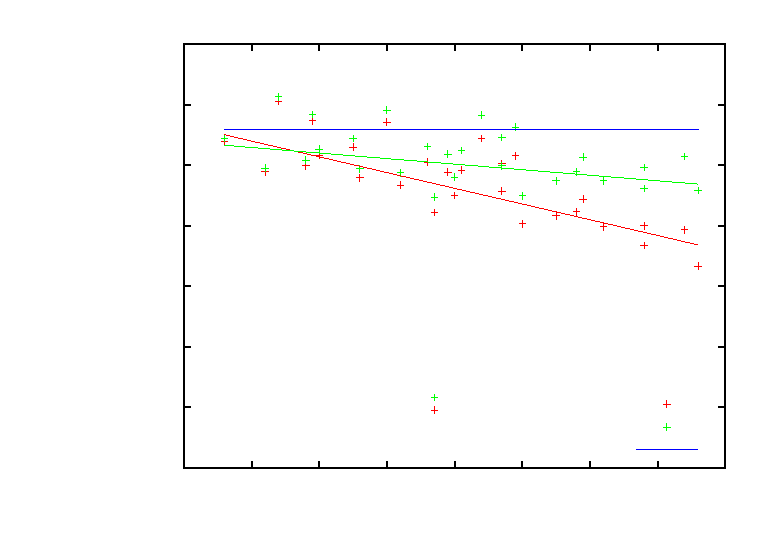
\includegraphics{ergebnisse}}%
    \gplfronttext
  \end{picture}%
\endgroup

\end{center}
\caption{Ergebnisse der Bestimmung der spezifischen Elektronenladung}
\label{fig:ergebnisse}
\end{figure}
Da die Abweichung des ermittelten Wertes mit $7.3\,\%$ außerhalb des ermittelten Fehlerbereichs liegt, scheinen die verwendeten Abschätzungen unzureichend zu sein.

Eine noch nicht betrachtete Fehlerquelle ist die Annahme des homogenen Magnetfeldes im Bereich des Glaskolbens.
Diese Näherung führt zu einer recht großen Abweichung, wie die Berechnung des Wertes mit elliptischen Integralen\footnote{per Wolfram Mathematica$^\text{\textregistered}$} zeigt. Die dafür benötigten Formeln wurden der Praktikumsanleitung \citep[S.~108]{Anleitung} entnommen.
Die relative Abweichung vom Literaturwert beträgt dann nur noch etwa $3.3\,\%$. Ein Vergleich der Ergebnisse ist in Abbildung~\ref{fig:ergebnisse} zu sehen. Auch gut zu erkennen ist die steigende Abweichung mit größerem Radius der Elektronenkreisbahn.
%Eine Berechnung des Fehlers per Gaußscher Fehlerfortpflanzung\footnote{mit Hilfe von Wolfram Mathematica$^\text{\textregistered}$} ergibt einen maximalen Messfehler von $\unit[?]{A}$.
Leider gestaltet sich die Berechnung der Gaußschen Fehlerfortpflanzung bei elliptischen Integralen äußerst schwierig, sodass darauf verzichtet werden musste.

Eine weitere Möglichkeit, die spezifische Elektronenladung aus den Messwerten zu bestimmen, ist das graphische Auftragen der Messwerte (siehe Abb.~\ref{fig:dUI-Kackplot}) mit anschließendem Ablesen der Steigung.
\begin{figure}[htb]
\begin{center}
\def\svgwidth{8cm}
% GNUPLOT: LaTeX picture with Postscript
\begingroup
  \makeatletter
  \providecommand\color[2][]{%
    \GenericError{(gnuplot) \space\space\space\@spaces}{%
      Package color not loaded in conjunction with
      terminal option `colourtext'%
    }{See the gnuplot documentation for explanation.%
    }{Either use 'blacktext' in gnuplot or load the package
      color.sty in LaTeX.}%
    \renewcommand\color[2][]{}%
  }%
  \providecommand\includegraphics[2][]{%
    \GenericError{(gnuplot) \space\space\space\@spaces}{%
      Package graphicx or graphics not loaded%
    }{See the gnuplot documentation for explanation.%
    }{The gnuplot epslatex terminal needs graphicx.sty or graphics.sty.}%
    \renewcommand\includegraphics[2][]{}%
  }%
  \providecommand\rotatebox[2]{#2}%
  \@ifundefined{ifGPcolor}{%
    \newif\ifGPcolor
    \GPcolortrue
  }{}%
  \@ifundefined{ifGPblacktext}{%
    \newif\ifGPblacktext
    \GPblacktextfalse
  }{}%
  % define a \g@addto@macro without @ in the name:
  \let\gplgaddtomacro\g@addto@macro
  % define empty templates for all commands taking text:
  \gdef\gplbacktext{}%
  \gdef\gplfronttext{}%
  \makeatother
  \ifGPblacktext
    % no textcolor at all
    \def\colorrgb#1{}%
    \def\colorgray#1{}%
  \else
    % gray or color?
    \ifGPcolor
      \def\colorrgb#1{\color[rgb]{#1}}%
      \def\colorgray#1{\color[gray]{#1}}%
      \expandafter\def\csname LTw\endcsname{\color{white}}%
      \expandafter\def\csname LTb\endcsname{\color{black}}%
      \expandafter\def\csname LTa\endcsname{\color{black}}%
      \expandafter\def\csname LT0\endcsname{\color[rgb]{1,0,0}}%
      \expandafter\def\csname LT1\endcsname{\color[rgb]{0,1,0}}%
      \expandafter\def\csname LT2\endcsname{\color[rgb]{0,0,1}}%
      \expandafter\def\csname LT3\endcsname{\color[rgb]{1,0,1}}%
      \expandafter\def\csname LT4\endcsname{\color[rgb]{0,1,1}}%
      \expandafter\def\csname LT5\endcsname{\color[rgb]{1,1,0}}%
      \expandafter\def\csname LT6\endcsname{\color[rgb]{0,0,0}}%
      \expandafter\def\csname LT7\endcsname{\color[rgb]{1,0.3,0}}%
      \expandafter\def\csname LT8\endcsname{\color[rgb]{0.5,0.5,0.5}}%
    \else
      % gray
      \def\colorrgb#1{\color{black}}%
      \def\colorgray#1{\color[gray]{#1}}%
      \expandafter\def\csname LTw\endcsname{\color{white}}%
      \expandafter\def\csname LTb\endcsname{\color{black}}%
      \expandafter\def\csname LTa\endcsname{\color{black}}%
      \expandafter\def\csname LT0\endcsname{\color{black}}%
      \expandafter\def\csname LT1\endcsname{\color{black}}%
      \expandafter\def\csname LT2\endcsname{\color{black}}%
      \expandafter\def\csname LT3\endcsname{\color{black}}%
      \expandafter\def\csname LT4\endcsname{\color{black}}%
      \expandafter\def\csname LT5\endcsname{\color{black}}%
      \expandafter\def\csname LT6\endcsname{\color{black}}%
      \expandafter\def\csname LT7\endcsname{\color{black}}%
      \expandafter\def\csname LT8\endcsname{\color{black}}%
    \fi
  \fi
  \setlength{\unitlength}{0.0500bp}%
  \begin{picture}(7200.00,5040.00)%
    \gplgaddtomacro\gplbacktext{%
      \csname LTb\endcsname%
      \put(1078,704){\makebox(0,0)[r]{\strut{} 0.05}}%
      \put(1078,1213){\makebox(0,0)[r]{\strut{} 0.06}}%
      \put(1078,1722){\makebox(0,0)[r]{\strut{} 0.07}}%
      \put(1078,2231){\makebox(0,0)[r]{\strut{} 0.08}}%
      \put(1078,2740){\makebox(0,0)[r]{\strut{} 0.09}}%
      \put(1078,3248){\makebox(0,0)[r]{\strut{} 0.1}}%
      \put(1078,3757){\makebox(0,0)[r]{\strut{} 0.11}}%
      \put(1078,4266){\makebox(0,0)[r]{\strut{} 0.12}}%
      \put(1078,4775){\makebox(0,0)[r]{\strut{} 0.13}}%
      \put(1210,484){\makebox(0,0){\strut{} 12}}%
      \put(2009,484){\makebox(0,0){\strut{} 14}}%
      \put(2808,484){\makebox(0,0){\strut{} 16}}%
      \put(3607,484){\makebox(0,0){\strut{} 18}}%
      \put(4406,484){\makebox(0,0){\strut{} 20}}%
      \put(5205,484){\makebox(0,0){\strut{} 22}}%
      \put(6004,484){\makebox(0,0){\strut{} 24}}%
      \put(6803,484){\makebox(0,0){\strut{} 26}}%
      \put(176,2739){\rotatebox{-270}{\makebox(0,0){\strut{}$d\,[\unit{m}]$}}}%
      \put(4006,154){\makebox(0,0){\strut{}$\sqrt{\frac{U}{\unit{1}{V}}}/\frac{I}{\unit{1}{A}}\,[\sim]$}}%
    }%
    \gplgaddtomacro\gplfronttext{%
      \csname LTb\endcsname%
      \put(5816,4602){\makebox(0,0)[r]{\strut{}Messwerte}}%
      \csname LTb\endcsname%
      \put(5816,4382){\makebox(0,0)[r]{\strut{}Lineare Regression}}%
    }%
    \gplbacktext
    \put(0,0){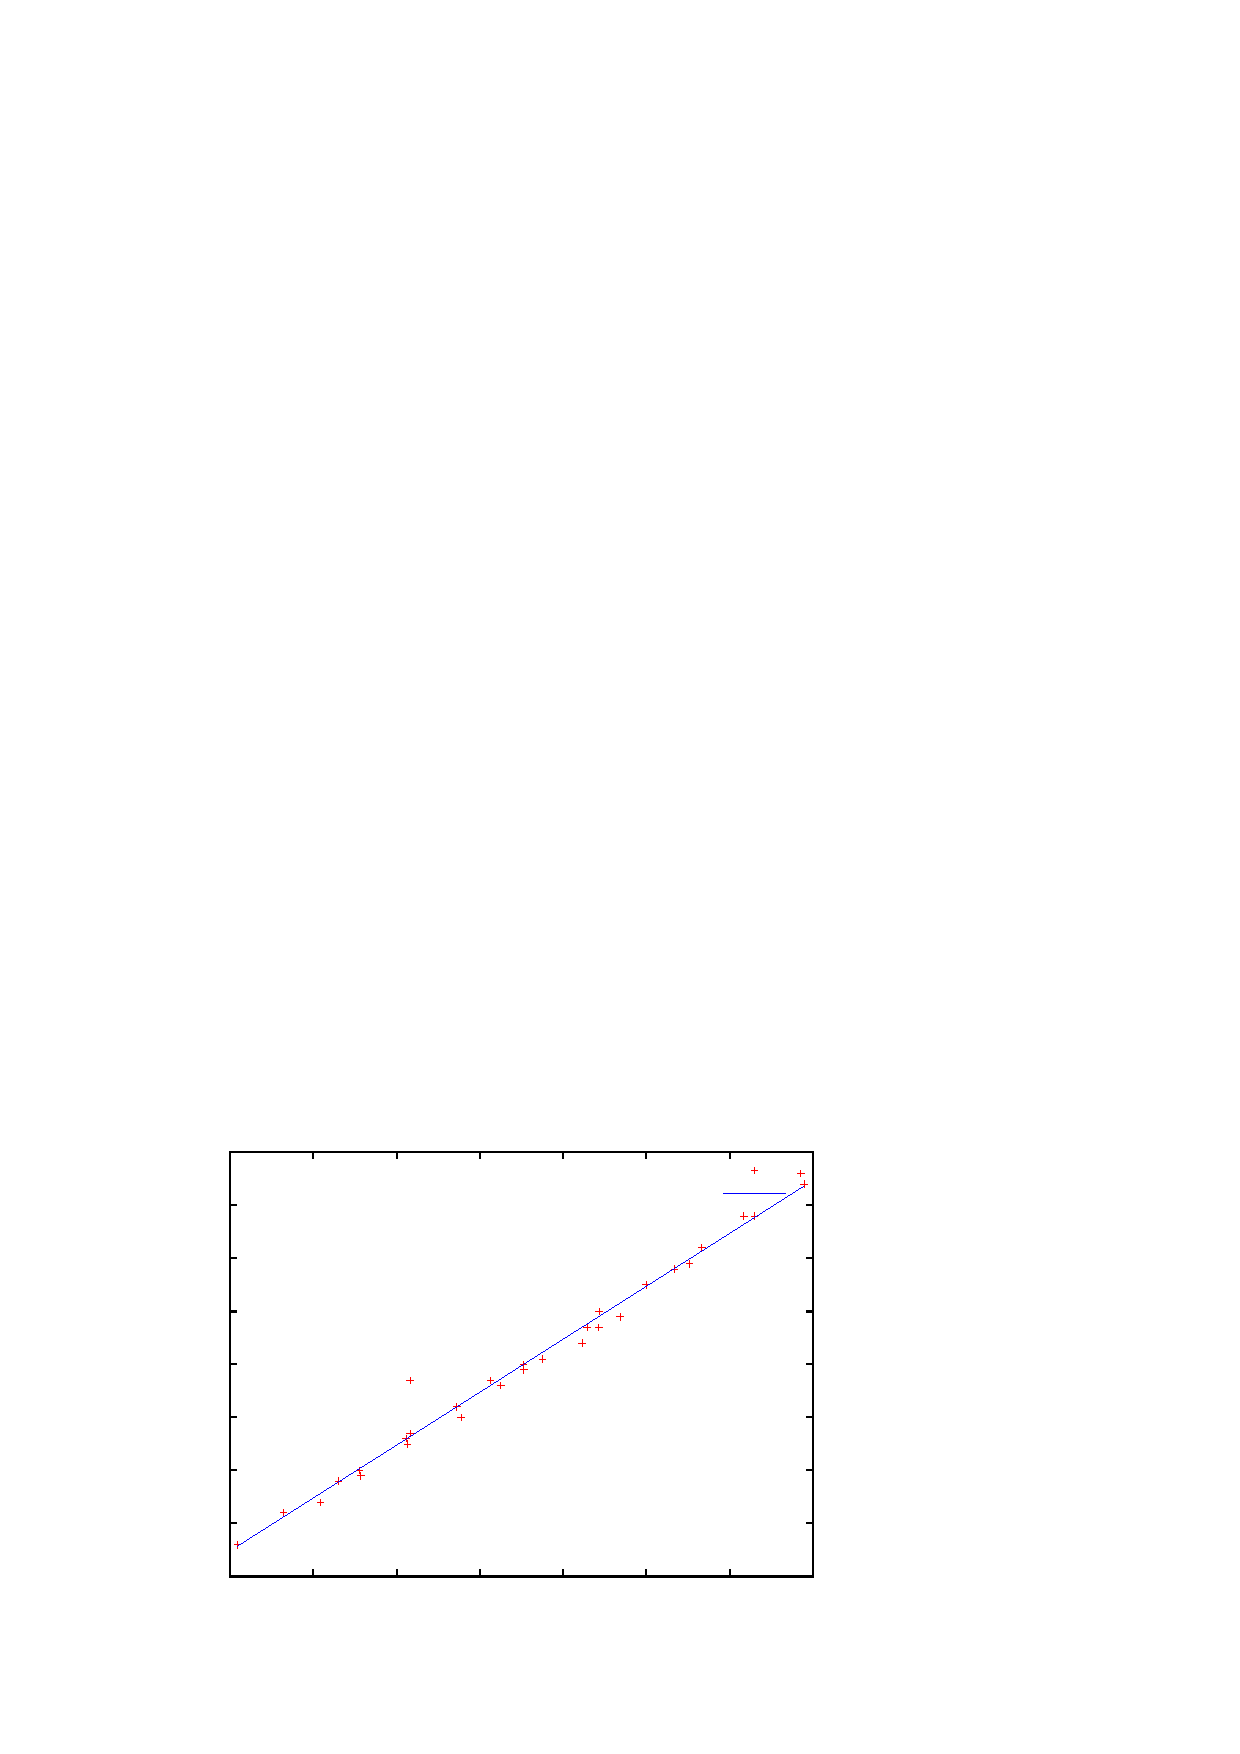
\includegraphics{edurchm}}%
    \gplfronttext
  \end{picture}%
\endgroup

\end{center}
\caption{Abhängigkeit des Elektronenstrahldurchmessers $d$ von dem Quotienten aus der Quadratwurzel der Spannung und der Stromstärke $\sqrt{U}/I$.}
\label{fig:dUI-Kackplot}
\end{figure}
Aus den Formeln~\ref{eq:B-Feld} und~\ref{eq:SpezLad} kann dann durch einfaches Umstellen und Einsetzen der Steigung ein Wert für die spezifische Ladung bestimmt werden.
Die relative Abweichung vom Literaturwert beträgt jedoch etwa $\unit[15.9]{\%}$.
Diese Berechnungsmethode führt also vermutlich zu sehr viel schlechteren Werten als die Berechnung mit Hilfe der einzelnen Wertepaare und anschließender gewichteter Mittelung.

Dies ist sehr erfreulich, da sich offenbar der sehr viel höhere Aufwand der anderen Methoden gelohnt hat.
Zum Vergleich der drei verwendeten Verfahren untereinander und mit dem Literaturwert siehe auch Tabelle~\ref{tab:Vergleich}.

Es fällt auf, dass die berechneten Werte unabhängig von der Rechenmethode eine Abweichung nach unten aufweisen.

Es scheint also ein systematischer Fehler in der Messung vorzuliegen.
Dieser könnte zur Ursache haben, dass der Versatz der Längenskala zur Messung des Strahldurchmessers nur einmal gemessen wurde.
Hier würde eine Abweichung des Messwertes nach oben die beobachteten Konsequenzen nach sich ziehen.
In Frage käme außerdem noch ein schwächeres Magnetfeld als berechnet oder eine stärkere Spannung als gemessen.
Letzteres ist aufgrund der hohen Genauigkeit der Multimeter jedoch recht unwahrscheinlich.


Weiterhin könnte eine etwaige Brechung des Lichts durch den Glaskolben zu kleineren Ungenauigkeiten führen.
Auch eine mögliche bei Verschiebung des Okulars auftretende kleine Drehung desselben um die vertikale Achse würde eine zusätzliche Abweichung zur Folge haben.

Einer der Messwerte (für $U_\mathrm{B} = \unit[140]{V},\,I = \unit[725]{mA}$) fällt vollkommen aus der Reihe und ist in allen Diagrammen deutlich zu erkennen. Wenn man anstatt der notierten $\unit[11.4]{cm}$ jedoch $\unit[10.4]{cm}$ einsetzt, ergibt sich ein deutlich besserer Wert, der statt $\unit[25.2]{\%}$ nur um $\unit[4.4]{\%}$ abweicht. Hier ist den Experimentatoren also offenbar ein Fehler unterlaufen.
 
\appendix
\newpage
\section{Tabellen und Grafiken}
\begin{table}[htb]
\centering
\begin{tabular}{|c|c|c|c|c|c|}
\hline
$U_B\,[\unit{V}]$ & $I\,[\unit{mA}]$ & $d\,[\unit{m}]$ & $B\,[\unit[10^{-3}]{T}]$ & $\nicefrac{e}{m_\mathrm{e}}\,[\unitfrac[10^{11}]{C}{Kg}]$ & $\nicefrac{e}{m_\mathrm{e}}_\mathrm{Ellipt.}\,[\unitfrac[10^{11}]{C}{Kg}]$ \\
\hline
200.0 & 550.0 & 0.126 & 0.811 & $1.53 \pm 0.08$ & 1.66 \\
\hline
200.0 & 614.0 & 0.109 & 0.905 & $1.64 \pm 0.09$ & 1.71 \\
\hline
200.0 & 678.0 & 0.097 & 0.999 & $1.70 \pm 0.10$ & 1.75 \\
\hline
200.0 & 742.0 & 0.089 & 1.094 & $1.69 \pm 0.11$ & 1.72 \\
\hline
200.0 & 806.0 & 0.080 & 1.188 & $1.77 \pm 0.12$ & 1.79 \\
\hline
200.0 & 870.0 & 0.075 & 1.282 & $1.73 \pm 0.13$ & 1.74 \\
\hline
200.0 & 934.0 & 0.069 & 1.377 & $1.77 \pm 0.14$ & 1.78 \\
\hline
200.0 & 998.0 & 0.064 & 1.471 & $1.80 \pm 0.15$ & 1.81 \\
\hline
120.0 & 450.0 & 0.118 & 0.663 & $1.57 \pm 0.09$ & 1.66 \\
\hline
120.0 & 525.0 & 0.100 & 0.774 & $1.60 \pm 0.10$ & 1.65 \\
\hline
120.0 & 600.0 & 0.087 & 0.884 & $1.62 \pm 0.11$ & 1.65 \\
\hline
120.0 & 675.0 & 0.076 & 0.995 & $1.68 \pm 0.13$ & 1.69 \\
\hline
120.0 & 750.0 & 0.068 & 1.106 & $1.70 \pm 0.14$ & 1.71 \\
\hline
120.0 & 825.0 & 0.062 & 1.216 & $1.69 \pm 0.15$ & 1.70 \\
\hline
120.0 & 900.0 & 0.056 & 1.327 & $1.74 \pm 0.17$ & 1.74 \\
\hline
120.0 & 575.0 & 0.090 & 0.848 & $1.65 \pm 0.11$ & 1.68 \\
\hline
140.0 & 575.0 & 0.097 & 0.848 & $1.66 \pm 0.10$ & 1.70 \\
\hline
160.0 & 575.0 & 0.105 & 0.848 & $1.62 \pm 0.09$ & 1.67 \\
\hline
180.0 & 575.0 & 0.112 & 0.848 & $1.60 \pm 0.09$ & 1.67 \\
\hline
200.0 & 575.0 & 0.118 & 0.848 & $1.60 \pm 0.08$ & 1.70 \\
\hline
220.0 & 575.0 & 0.124 & 0.848 & $1.59 \pm 0.08$ & 1.71 \\
\hline
170.0 & 575.0 & 0.108 & 0.848 & $1.62 \pm 0.09$ & 1.69 \\
\hline
120.0 & 725.0 & 0.070 & 1.069 & $1.72 \pm 0.14$ & 1.73 \\
\hline
140.0 & 725.0 & 0.087 & 1.069 & $1.30 \pm 0.09$ & 1.32 \\
\hline
160.0 & 725.0 & 0.082 & 1.069 & $1.67 \pm 0.12$ & 1.69 \\
\hline
180.0 & 725.0 & 0.086 & 1.069 & $1.70 \pm 0.11$ & 1.73 \\
\hline
200.0 & 725.0 & 0.091 & 1.069 & $1.69 \pm 0.11$ & 1.72 \\
\hline
220.0 & 725.0 & 0.094 & 1.069 & $1.74 \pm 0.11$ & 1.78 \\
\hline
240.0 & 725.0 & 0.099 & 1.069 & $1.72 \pm 0.10$ & 1.76 \\
\hline
\end{tabular}
\caption{Aus den Messwerten per Wolfram Mathematica$^\text{\textregistered}$ mit elliptischen Integralen numerisch bestimmte Magnetfeldstärken sowie die bestimmten spezifischen Elektronenladungen.}
\label{tab:Feldstaerke}
\end{table}
\begin{table}[htb]
\centering
\begin{tabular}{|c|c|c|}
  \hline
  Berechnungsmethode & $e/m_e\,[\unit{C/kg}]$ & rel. Abweichung vom Lit.-Wert $[\%]$\\
  \hline
  Gewichtetes Mittel (Ell. Int.) & $1.701$ & $-3.3$ \\
  \hline
  Gewichtetes Mittel (Standard) & $1.631 \pm 0.018$ & $-7.3$\\
  \hline
  Regression & $1.478 \pm 0.071$ & $-15.9$ \\
  \hline
\end{tabular}
\caption{Vergleich der verwendeten Verfahren, Literatur: $e/m_e \approx \unit[1.759\cdot10^{11}]{C/kg}$.}
\label{tab:Vergleich}
\end{table}
 
\bibliographystyle{dinat}
\newpage
\bibliography{../Shared/bibliography.bib}
\end{document} 
